\chapter{Eksperyment LHCb}

Badania opisywane w niniejszej pracy zostały wykonane w Europejskim Ośrodku Badań Jądrowych (CERN) pod Genewą. Laboratorium zostało założone w 1954 roku i zrzeszało 12 Europejskich krajów. Wartą odnotowania data jest 1 lipca  1991 roku, kiedy to Polska stała się pełnoprawnym członkiem CERN. Międzynarodowa kolaboracja była i jest jedynym sensownym rozwiązaniem problemów ze zwiększającymi się wymaganiami co do złożoności oraz kosztów prowadzenia eksperymentów fizyki wysokich energii.

Analizowane pomiary zostały przeprowadzone przy użyciu akceleratora zwanego Wielkim Zderzaczem Hadronów (ang. Large Hadron Collider) oraz eksperymentu LHCb. Rozdział ten ma na celu dać krótkie wprowadzenie do zagadnień związanych z eksperymentem w k  pracach którego, autor bierze czynny udział. 

\section{Akcelerator LHC}
\indent LHC jest największym, działającym akceleratorem na świecie zaprojektowanym do zderzania protonów o całkowitej energii środka masy $\sqrt{s}=14 TeV$. Poza samą energia wiązki ważnym parametrem związanym z pracą akceleratora jest  świetlność ($L$). Wielkość ta określa ile zaszło zderzeń cząstek, kiedy dwie wiązki zderzyły się ze sobą. Co więcej liczba ta jest ściśle związana z ilością zderzeń na sekundę oraz przekrojem czynnym:
\begin{equation}
\frac{dN}{dt} =L \sigma
\end{equation}
Ilość zebranych danych można otrzymać całkując chwilową świetlność:
\begin{equation}
\mathcal{L} = \int L dt
\end{equation}
Otrzymana wielkość posiada jednostkę odwrotności pola, zwaną również barnem. Eksperymenty ATLAS oraz CMS (opisane poniżej) mogą pracować z maksymalną osiągalną świetlnością przez LHC-$\mathcal{L}=10^{34}cm^{-2}s^{-1}$, natomiast LHCb dla swoich potrzeb redukuje świetlność w celu zmniejszenia ilości wielokrotnych zderzeń na wiązkę. 

LHC został umiejscowiony w 26,7 km tunelu skonstruowanym pierwotnie dla poprzedniego akceleratora elektronowego LEP (ang. Large Electron–Positron Collider). 
\begin{figure}[h]
  \centering
  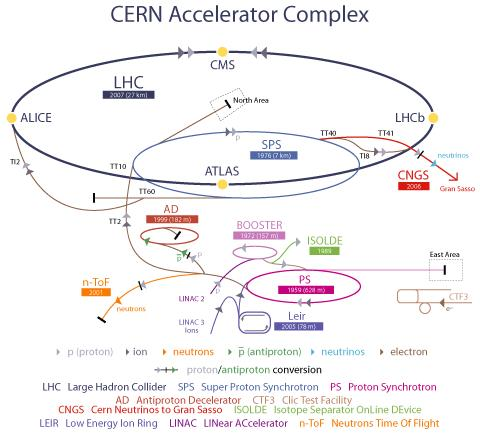
\includegraphics[scale=1]{rozdzial2/AccComple.jpeg}
  % AccComple.gif: 480x434 pixel, 72dpi, 16.93x15.31 cm, bb=0 0 480 434
  \caption{Schemat kompleksu przyspieszającego akceleratora LHC. \cite{public}}
  \label{fig:AccComplex}
\end{figure}

Na rysunku \ref{fig:AccComplex} pokazany jest schemat kompleksu przyspieszającego oraz detektorów pracujących przy eksperymencie LHC. Sam proces przyspieszania jest kilku stopniowy\cite{Haefeli}.
Na początku protony otrzymywane są w wyniku jonizacji atomów wodoru po czym wstępnie przyspieszane w akceleratorze liniowym (LINIAC2) do energii 500MeV. Następnie dwa kołowe akceleratory zwiększają energie cząstek do 1GeV (BOOSTER) oraz 26 GeV (PS), kontynuując podróż przez system akceleratorów  przechodzą przez SPS rozpędzający je do energii 450 GeV. Na sam koniec są umieszczane w docelowym pierścieniu LHC. W którym to przebywają 20 minut zanim nabiorą maksymalną energię. Do utrzymania dwóch przeciwbieżnych wiązek protonowych na ich orbitach potrzebne są 1232 nadprzewodzące magnesy, generujące pole o indukcji 8.33T. Aby magnesy pozostawały w stanie nadprzewodzenia muszą być schłodzone do temperatury 1.9 K. Tak niską temperaturę uzyskuje się przy użyciu nadciekłego helu. 

Wiązki są zderzane w 4 punktach oznaczonych na rysunku \ref{fig:AccComplex} żółtymi kropkami. W każdym z tych punktów umiejscowiony jest jeden z detektorów oraz powiązanych z nimi eksperyment. Noszą one odpowiednio nazwy ATLAS, CMS, ALICE oraz LHCb.

Głównymi celami eksperymentów ATLAS (ang. A Toroidal Lhc ApparatuS)\cite{ATLAS} oraz CMS (ang. Compact Muon Solenoid) \cite{CMS} jest poszukiwanie bozonu Higgsa, cząstki która wg Modelu Standardowego odpowiada za nadawanie masy, oraz sprawdzenie teorii supersymetrii (SUSY). ALICE (ang. A Large Ion Collider Experiment)\cite{ALICE} został zoptymalizowany do badania plazmy gluonowo-kwarkowej powstającej w wyniku zderzeń ciężkich jonów.


\section{Detektor LHCb}
Eksperyment oraz stowarzyszony z nim detektor LHCb został zaprojektowany do badania łamania symetrii kombinowanej \textbf{CP} oraz rzadkich procesów obficie produkujących hadrony zawierające kwarki b. Jako przykład można podać mezon B. Produkcja pary $b\overline{b}$ będąca wynikiem zderzenia proton-proton jest zdominowana przez procesy fuzyjne gluonów i partonów, diagram Feynmana opisujący takie procesy został umieszczony na rysunku \ref{fig:feynman}.  Symulacje takich procesów pokazały, że przy energiach osiąganych dzięki LHC, zarazem kwarki b oraz $\overline{b}$ przeważnie produkowane są w kierunku do przodu lub tyłu, co przedstawiono na rysunku\ref{fig:pythia}.  


\begin{figure}[h]
  \centering
  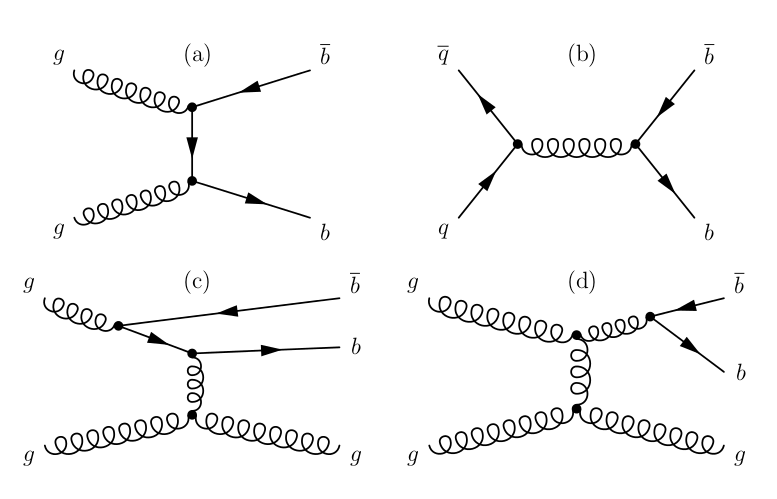
\includegraphics[scale=0.5]{rozdzial2/Feynman.png}
  % AccComple.gif: 480x434 pixel, 72dpi, 16.93x15.31 cm, bb=0 0 480 434
  \caption{Przykładowe diagramy Feynmana obrazujące produkcję mezonów B. Diagramy pierwszego rzędu odpowiadają kreacji par przez fuzję gluonową (a) oraz anihilację kwark-antykwark(b). Przykładowe schematy wyższych rzędów to wzbudzenia zapachowe (c) oraz rozszczepianie gluonu}
  \label{fig:feynman}
\end{figure}



\begin{figure}[h]
  \centering
  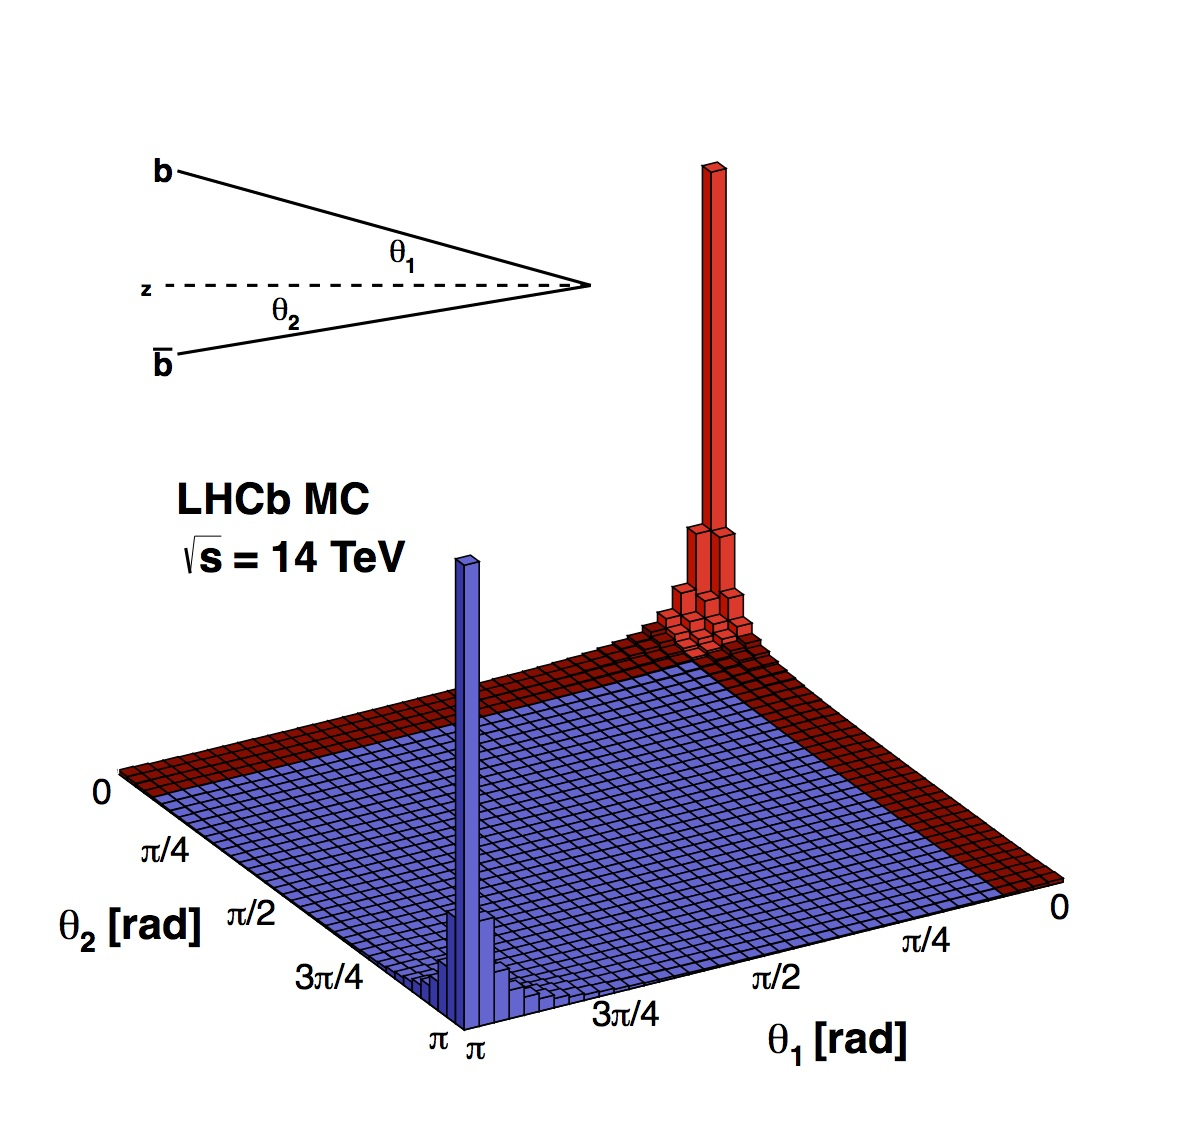
\includegraphics[scale=0.5]{rozdzial2/pythia.jpg}
  % AccComple.gif: 480x434 pixel, 72dpi, 16.93x15.31 cm, bb=0 0 480 434
  \caption{Wykres korelacji pomiędzy kątem polarnym a ilością produkowanych kwarków b w zderzeniu proton-proton. Symulacja została wykonana przy użyciu programu Pythia \cite{public}}
  \label{fig:pythia}
\end{figure}

Detektor LHCb jest spektrometrem o akceptanci kątowej 10 do 300 mrad. Jest to geometria typu "do przodu", której konsekwencją jest efektywny przedział pseudorapidity obserwowanych cząstek\\ $1.7<\eta < 5.3$ . Przy czym pseudorapidity, $\eta $ jest zdefiniowana jako
\begin{equation}
 \eta=-\ln\left(\tan\frac{\theta}{2}\right)
\end{equation}
gdzie $\theta$ kąt między kierunkiem pędu cząstki oraz osią wiązki.


\begin{figure}[h]
  \centering
  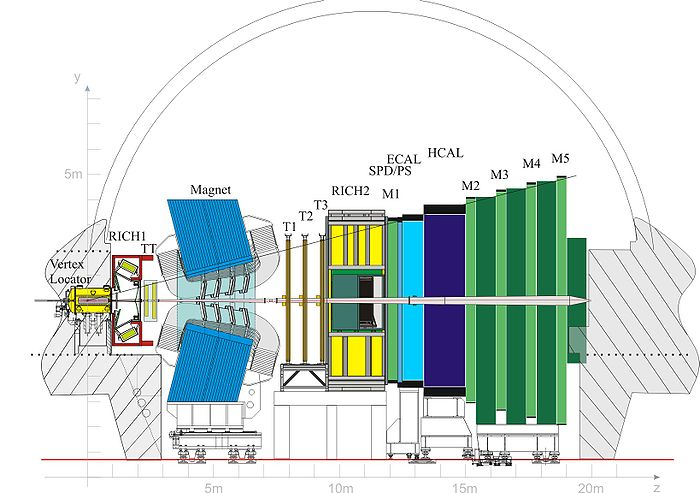
\includegraphics{rozdzial2/Lhcbview.jpg}
  % Lhcbview.jpg: 700x493 pixel, 150dpi, 11.85x8.35 cm, bb=0 0 336 237
  \caption{Schemat detektora LHCb \cite{public}}
  \label{fig:Layout}
\end{figure}

Zamieszczony na rysunku \ref{fig:Layout} spektrometr LHCb składa się z szeregu systemów detekcyjnych, które będą opisane w dalszej części rozdziału. 

\subsection{Detektory Czerenkowa}
RICH (ang. Ring Imaging Cherenkov detector) jest detektorem promieniowania Czerenkowa wykorzystywanym do identyfikacji hadronów. W szczególności wydajna separacja pionów oraz kaonów jest niezbędna przy badaniu rozpadów mezonów $B_{(s)}^0$ oraz $D_{(s)}^0$. W spektrometrze LHCb zamontowano dwa detektory RICH. Pierwszy z nich (RICH1), umieszczony zaraz za VELO, jest zoptymalizowany dla nisko pędowych cząstek o pędzie w przedziale $\sim 1- 60 GeV/c$. Drugi (RICH2), położony za magnesem, służy do identyfikacji cząstek o dużych pędach ($\sim 15-100 GeV/c$) \cite{RICH}. Zasada działania wyżej wymienionych detektorów jest oparta na procesie emisji promieniowania Czerenkowa. Promieniowanie to jest emitowane gdy naładowana cząstka porusza się w danym ośrodku szybciej niż światło w tym ośrodku. Kąt emitowanego fotonu jest zależny od prędkości z jaką porusza się cząstka wg wzoru
\begin{equation}
 cos\theta=\frac{c}{n v}
\end{equation}
gdzie:\\
c- prędkość światłą w próżni, v- prędkość cząstki, n- współczynnik załamania ośrodka.
\subsection{Detektory śladowe}
Układ detektorów śladowych pozwala na rekonstrukcję trajektorii cząstek oddziałujących z materiałem czynnym detektora. Składa się z części umieszczonych przed magnesem (VELO, TT) oraz za nim (stacje T1-T3 oraz komory mionowe). Ze względu na temat pracy, bezpośrednio związany z detektorem VELO, zostanie on dokładnie opisany w rozdziale \ref{VELO}. Umieszczony na rysunku \ref{fig:TTlayout} TT (ang. Tracker Turicensis) jest wykorzystywana w analizie do rekonstrukcji długożyciowych neutralnych cząstek np. kaonów rozpadających się na zewnątrz detektora VELO. Detektor ten zbudowany jest z czterech warstw krzemowych, mikropaskowych detektorów. 
\begin{figure}[th]
  \centering
  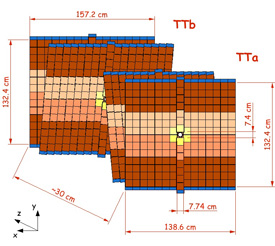
\includegraphics[scale=1]{rozdzial2/TT-layout.jpg}
  % TT-layout.jpg: 275x246 pixel, 100dpi, 6.99x6.25 cm, bb=0 0 198 177
  \caption{Schemat detektor TT \cite{public}}
  \label{fig:TTlayout}
\end{figure}
Detektory śladowe T1-T3,których schemat zamieszczono na rysunku \ref{fig:OTLayput},  dokonujące pomiarów pozycji za magnesem, dzielą się na dwie części. Pierwszą z nich jest IT (ang. Inner Tracker) zbudowany podobnie jak TT, z krzemowych mikropaskowych detektorów. Wynika to z faktu iż IT znajduje się w miejscu którym oczekiwane jest największa ilość cząstek, natomiast OT(ang. Outer Tracker) jest gazowym detektorem słomkowym.

\begin{figure}[th] 
  \centering
  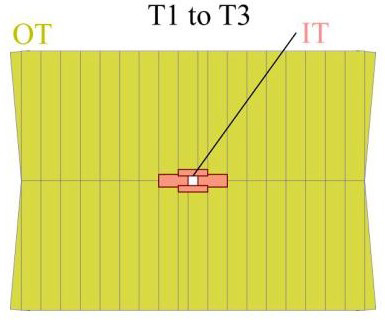
\includegraphics[scale=0.5]{rozdzial2/OT-Module-design.jpg}
  % OT-Module-design.jpg: 385x326 pixel, 100dpi, 9.78x8.28 cm, bb=0 0 277 235
  \caption{Schemat detektorów T1-T3\cite{public}}
  \label{fig:OTLayput}
\end{figure}

\subsection{Kalorymetry}
Zadaniem  kalorymetrów jest identyfikacja fotonów, elektronów i hadronów oraz pomiar ich energii. Są wykorzystywane również w algorytmie systemu wyzwalania. System dzieli się na kilka części:
\begin{itemize}
\item SPD (ang. Scintillator Pad Detector) oraz PS (ang. Pre Shower) służą do odróżniania fotonów i elektronów poprzez analizę topologii elektromagnetycznej kaskady cząstek wtórnych.
\item ECAL (ang. Electromagnetic CALorimeter) mierzy energię fotonów i elektronów. 
\item HCAL (ang. Hadronic CALorimeter) używany do pomiaru energii hadronów.
\end{itemize}
\subsection{Komory mionowe}
Identyfikacja mionów jest fundamentalnym wyzwaniem eksperymentu LHCb ponieważ cząstki te są stanami końcowymi powstającymi w wyniku rozpadów mezonów $B_{(s)}^0$ oraz $D_{(s)}^0$ . Miony, słabo oddziaływające z materią, są jedynymi cząstkami które przechodzą przez system kalorymetrów. Układ detektorów składa się z pięciu wielodrutowych komór proporcjonalnych. Mają bardzo ważną rolę w systemie wyzwalania L0, oraz estymacji pędu poprzecznego mionów.
\subsection{System wyzwalania}
Częstotliwość przecinania się wiązek protonowych wynosi 40MHz, co w przybliżeniu odpowiada strumieniowi danych 40TB/s. W celu ograniczenia strumienia danych zastosowano system wyzwalania (ang. trigger). Obecny system akwizycji jest w stanie archiwizować dane przychodzące z prędkością nie większą niż 200 MB/s(4kHz). Końcowy efekt uzyskany jest dzięki dwóm poziomom decyzyjnym.
\begin{itemize}
 \item Pierwszy poziom (Level0 [L0]) ogranicza  strumień danych z 40 MHz do 1.1MHz. Wykorzystuje on w procesie dokonywania decyzji fakt iż produkty rozpadów mezonów $B_{(s)}^0$ oraz $D_{(s)}^0$ posiadają stosunkowo wysoki pęd poprzeczny oraz energię. 
 \item Drugi poziom (High Level Trigger [HLT]) jest programem komputerowym wykonywanym na bardzo wielu CPU jednocześnie. Wykorzystuje dane pochodzące ze wszystkich detektorów. Szybki algorytm rekonstrukcji śladów łączy wyniki pochodzące z VELO wraz ze śladami zrekonstruowanymi przez inne detektory śladowe. Na tej podstawie wybiera się przypadki fizyczne, które zapisywane są na dysku.  
\end{itemize}
\begin{figure}[ht]
  \centering
  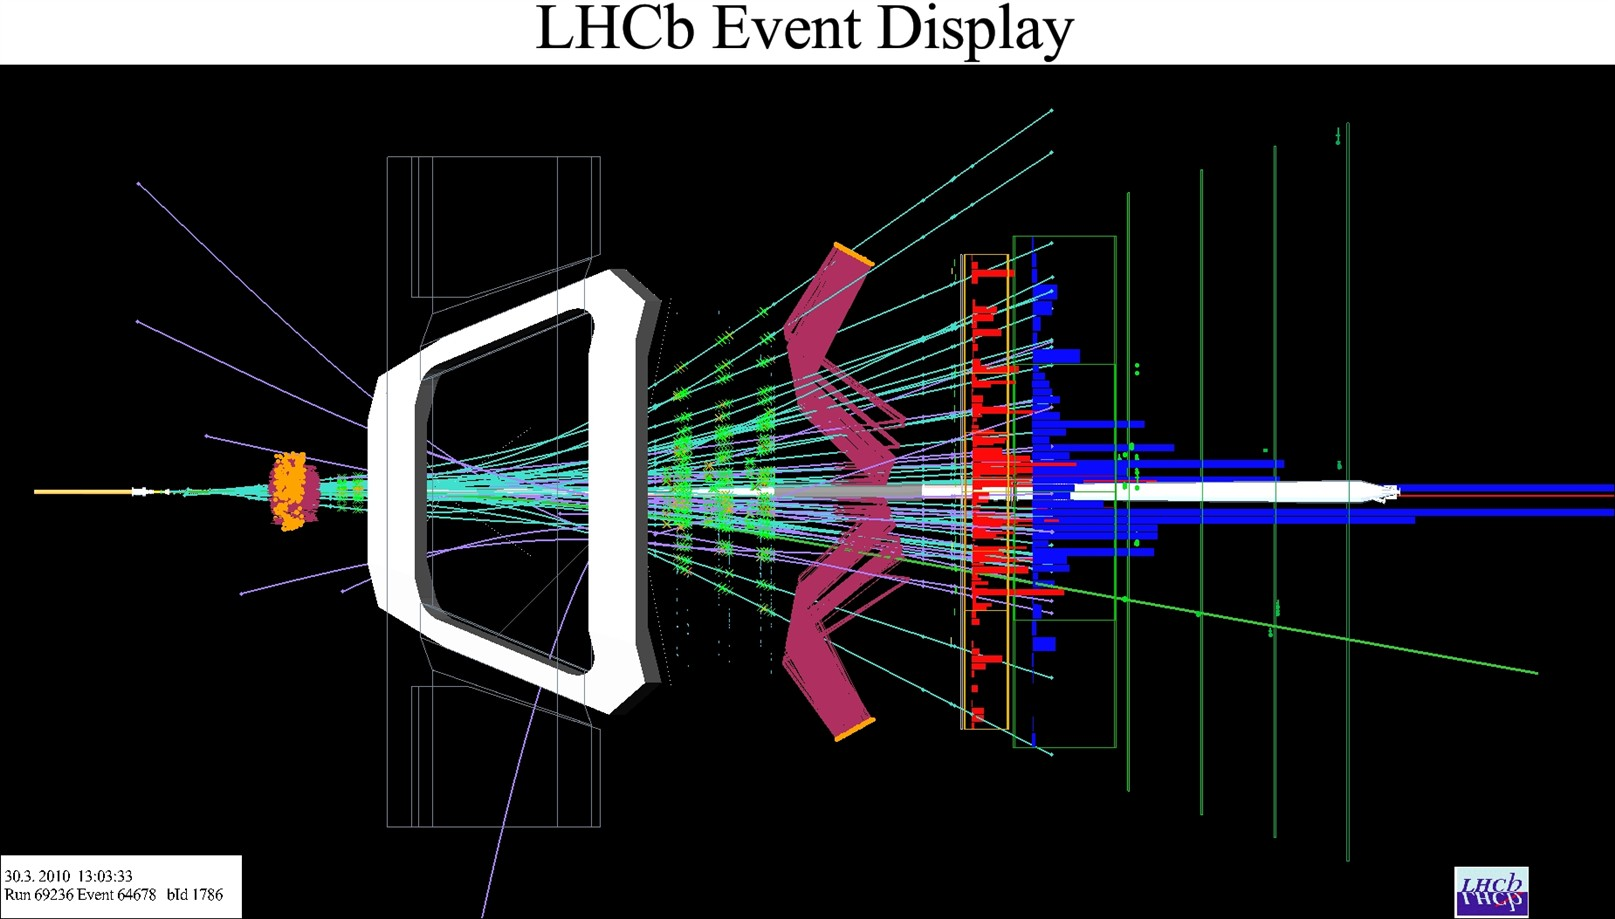
\includegraphics[scale=0.5]{rozdzial2/event.jpg}
  % event.jpg: 1615x919 pixel, 144dpi, 28.49x16.21 cm, bb=0 0 808 460
  \caption{Wizualizacja przypadku zdarzenia w detektorze LHCb\cite{event}}
  \label{fig:event}
\end{figure}
